
\documentclass{article}

%%%%%%%%%%%%%%% LIBRERIAS %%%%%%%%%%%%%%%%%%%%%
\usepackage{amsmath}
\usepackage{titlesec}
\usepackage{titletoc}
\usepackage{graphicx}
\usepackage[spanish,es-tabla]{babel} % 'es-tabla' cambia Cuadro→Tabla
\usepackage{hyperref}                % cargar después de babel
\usepackage{float}
\usepackage{circuitikz}
\usepackage[a4paper, margin=3cm]{geometry}
%%%%%%%%%%%%%%%%%%% VARIABLES %%%%%%%%%%%%%%%%%%%%
\newcommand{\Facultad}{Instituto Tecnológico \\de\\ Buenos Aires} %constantes
\newcommand{\TPn}{Trabajo Práctico N° 1}
\newcommand{\TPtema}{Corriente Continua}
\renewcommand{\thesection}{\arabic{section}}          % 2
\renewcommand{\thesubsection}{\quad \alph{subsection}}   % a
\renewcommand{\thesubsubsection}{\quad \thesubsection.~\roman{subsubsection}} % a. i
\graphicspath{{imagenes&matlab/}} %para que acceda a las fotos en la carpeta directamente


%%%%%%%%%%%%%%%%%% FORMATO TÍTULO Y NUMERACIÓN %%%%%%%%%%%%%%%%%%%
% Numeración de secciones
\renewcommand{\thesection}{\arabic{section}.}          
\renewcommand{\thesubsection}{\thesection\arabic{subsection}}       
\renewcommand{\thesubsubsection}{$\alph{subsubsection})$}

% Numerar hasta subsubsecciones
\setcounter{secnumdepth}{3}

% Formato de títulos
\titleformat{\section}{\Huge\bfseries}{\thesection}{1em}{}
\titleformat{\subsection}{\LARGE\bfseries}{\thesubsection}{0.5em}{}
\titleformat{\subsubsection}{\large\bfseries}{\thesubsubsection}{0.5em}{}



%%%%%%%%%%%%%%%%%%% ARCHIVO %%%%%%%%%%%%%%%%%%%%%%%%
\begin{document}

    %%%CARATULA%%%
    \begin{titlepage} %creo portada

        \begin{flushleft}
            \centering
            
\includegraphics[width=0.3\textwidth]{Logo_ITBA.png}
        \end{flushleft}

        \centering
            
        {\scshape\LARGE \Facultad \par} %\par sirve para indicar un final de parrafo
        \vspace{1cm}                    %esto hace un espacio entre lineas de 1cm


        {\huge\bfseries \TPn \par}
        \vspace{1.5cm}
        {\Large Teoría de Circuitos I\\ 25.10 \par}
        \vfill                      %sirve para rellenar el espacio y quede simétrico. Si se añaden otros, se dividen el espacio de forma equitativa
        {\Large \bfseries Grupo N° 5 \par}
        \vspace{1cm}
        {\large Juan Bautista Correa Uranga \hfill Legajo: 65016 \par} %\hfill sirve para hacerlo simétrico
        {\large Juan Ignacio Caorsi \hfill Legajo: 65532  \par}
        {\large Rita Moschini \hfill Legajo: 67026 \par} 
        \vfill
        {\large \today\par}
        \vfil

    \end{titlepage}


    %%%RESUMEN%%%
    {\centering \LARGE \bfseries Resumen \par}

    \newpage

    %%%INDICE%%%
    \tableofcontents %esto sirve para crear el índice
    \newpage

    %%%Introduccion%%%
    \section{Introducción}

        Para esta practica se usó corriente alterna para el estudio de la potencia en AC. 
    

        \subsection{Instrumental}

        En esta experiencia se utilizaron los siguientes instrumentos:

        \begin{itemize}
            \renewcommand{\labelitemi}{$\bullet$}
            \item {\bfseries Variac}: Fuente de tensión AC regulable. 
            \item {\bfseries Vatímetro analógico}: El mismo sirve para poder medir la potencia activa (P) consumido por el circuito.
                    Para calcular los valores, el mismo debe medir la tensión y la corriente del circuito. Para ello se conecta de la siguiente forma (observar figura). \par
                
            \item {\bfseries Amperímetro analógico}
            \item {\bfseries Voltímetro analógico}
            \item {\bfseries Inductor}: Consta de un armazón plastico hueco, al cual se le enrrolla un alambre sucesivas veces. El mismo tiene asociado una resistencia y un valor L inductivo. 
                Este tenía un hueco en el medio donde se podía intrucir un nucleo de material sólido. 
        \end{itemize}
        
        \subsection{Marco teórico}

        En esta practica se usaron los siguientes conocimientos teoricos:

        \subsubsection{Inductor}

        Como se mencionó anteriormente, un inductor consta de un alambre enrrollado. El mismo es capaz de almacenar energía electrica en forma de energía magnética.
         La ecuación del mismo viene dada por:
        \begin{equation*}
            V=L \frac{dI}{dT}
        \end{equation*}
        De esta ecuacion se puede deducir que el inductor no puede tener cambios bruscos en la corriente de un instante al otro, por lo que debe ser continua en todo instante.

        Usando cambio de variable a números complejos, se puede llegar a la siguiente ecuación.
        \begin{equation*}
            V=j\cdot \omega\cdot L
        \end{equation*}
        con j la constante compleja, $\omega$ la frecuencia en $\frac{rads}{seg}$ y L la constante inductiva en H.

        \subsubsection{Potencia compleja}

        Al analizar la potencia asociada a circuitos AC, se debe tener en consideración los siguientes aspectos.\par
        La potencia total se llama { \bfseries potencia compleja} $\vec{S}= V \cdot I^{*}$ [VA], y es la potencia total del sistema. No obstante, es importante mencionar que este número no representa la potencia total usada por el sistema.
        La potencia compleja se puede describir de la siguiente forma $\vec{S}=P + j \cdot Q$, donde P es la { \bfseries potencia activa} y Q es la {\bfseries potencia reactiva}. \par

        La potencia activa (P) es la potencia que es efectivamente usada por el sistema. Esta representa la parte real de la potencia compleja.
        Más aun, la misma se puede descomponer en $P= |I_{rms}| \cdot |V_{rms}| \cdot \cos (\varphi)$. De esto se puede deducir lo siguiente, la misma es máxima cuando el desfasaje $\varphi = \theta_{V} - \theta_I $ es cero. \par

        Por otra parte, la potencia reactiva es la parte imaginaria de $\vec{s}$. Esta representa la potencia inductiva o capacitiva. Esta se puede descomponer en $ Q = |I_{rms}| \cdot |V_{rms}| \cdot \sen (\varphi)= \pm \frac{V_\text{rms}^2}{X}$ donde es + si es inductivo o - si es capacitivo.
        De esta formula se puede deducir que el mismo es minimo cuando el desfasaje entre la corriente y la tension se acerca a cero, 
        la potencia reactiva se reduce. La potencia reactiva, a diferencia de la potencia activa, es una potencia la cual no puede ser aprovechada por el sistema, 
        ya que la misma esta asociada (como se pudo observar en la ecuacion que la define) a la energia almacenada por los inductores y los capacitores.\par

        En consecuencia, este último tipo de potencia se suele reducir al mínimo posible, por motivos económicos.

        Por último, P y Q se pueden relacionar usando el triangulo de potencia (observar Figura \ref{fig:triangulo_de_potencia}). 
        \begin{figure}[h!] % h! = aquí, lo más forzado posible
            \centering
            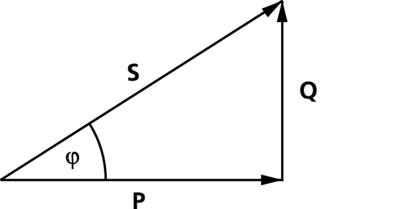
\includegraphics[width=0.5\textwidth]{Trojkat-mocy.png} % nombre del archivo
            \caption{Triangulo de potencia inductivo}
            \label{fig:triangulo_de_potencia} % etiqueta para referencias
        \end{figure}

    %%%Desarrollo%%%
    \indent
    \section{Desarrollo}

    \subsection{Procedimiento}
   
    %%%Conclusiones%%%
    \section{Conclusiones}

    %%%Anexos%%%
    \section{Anexos}

\end{document}